\beginsong{Tief im Busch}[wuw={Kurt Feltz, Peter Laine, 1966}]

\beginverse
\endverse
\centering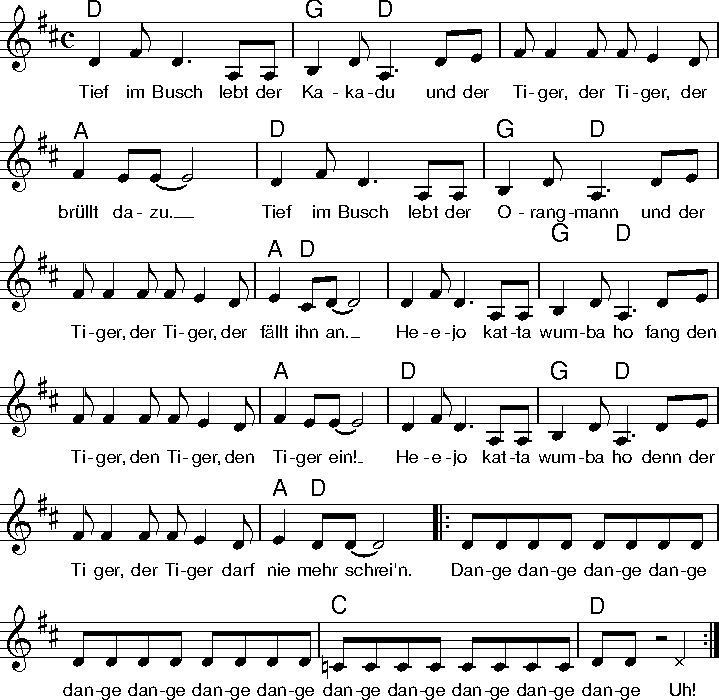
\includegraphics[width=1\textwidth]{Noten/Lied084.pdf}

\beginverse
\[D]Keine Nacht ist der \[G]Urwald \[D]still, 
weil der Tiger, der Tiger nicht \[A]schlafen will.
\[D]Keine Nacht ist der \[G]Urwald \[D]stumm,
denn der Tiger, der Tiger, der \[A]schleicht \[D]herum.
\endverse

\beginchorus
He-e-jo katta \[G]wumba \[D]ho, 
fang den Tiger, den Tiger, den \[A]Tiger ein!
\[D]He-e-jo katta \[G]wumba \[D]ho, 
denn der Tiger, der Tiger darf \[A]nie \[D]mehr schrei'n.
\lrep \[D]Dange dange dange dange dange dange dange dange, \[C]dange dange dange dange, \[D]uh. \rrep
\endchorus

\beginverse
^Weißer Mann mit dem ^Schießge^wehr,
macht dem Tiger, dem Tiger, das ^Leben schwer.
^Weißer Mann in der ^letzten ^Nacht,
hat der Tiger, der Tiger dich ^um^gebracht.
\endverse
\renewcommand{\everychorus}{\textnote{\bf Refrain (wdh.)}}
\beginchorus
\endchorus

\endsong
